\documentclass[border=0bp]{standalone}
\usepackage[T1]{fontenc}
\usepackage{newpxtext,newpxmath,graphicx,tikz}
\begin{document}
\begin{tikzpicture}[x=1bp,y=-1bp]
\path[use as bounding box] (0,0) rectangle (859,328);
\node[anchor=north west,inner sep=0pt] at (0,0) {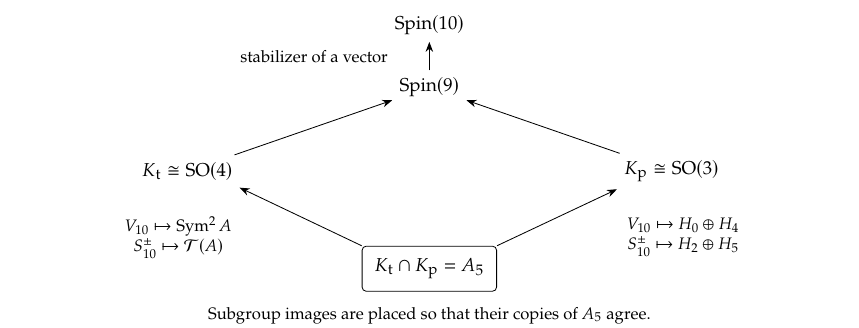
\includegraphics[width=859bp,height=328bp]{fig03_spin_intersection_original.png}};
\fill[white] (42,299) rectangle (825,327);
\node[anchor=north,inner sep=0pt,text width=780bp,align=center,font=\fontsize{15bp}{18bp}\selectfont] at (429.5,304) {The two subgroup embeddings are chosen to contain the same copy of $A_5$.};
\end{tikzpicture}
\end{document}
